\newpage
\section{Designing for Manufacturability and Feasibility Audits}
\label{app:details}
We report on hardware setup and hyperparameter details for full reproducibility. In addition, we also provide more examples of chip designs discovered by our method that are of interest. 


\subsection{Five Levels of Validation}
\label{app:validation}
We validate the physical manufacturability and feasibility of our framework at four levels.

\begin{enumerate}
    \item Roofline Auditor: A deterministic Roofline Auditor checks physical feasibility by comparing
each LP-predicted latency against the lower bound
\begin{equation}
    \mathrm{LB} = \max\!\left(t_{\mathrm{compute}},\;
    t_{\mathrm{memory}}\right),
\end{equation}
where $t_{\mathrm{compute}}$ is total FLOPs divided by peak FLOPs/s and
$t_{\mathrm{memory}}$ is post-placement off-chip traffic divided by
available memory bandwidth.
The audit additionally reports $\mathrm{MFU}_{\mathrm{bound}}$ and memory
utilization; values above 1 would indicate a physically impossible
prediction.
All results withing this paper are roofline-feasible with zero lower-bound violations, and~\cref{app:mfu} gives more details.

\item Campaign Validator: A deterministic Campaign Validator legalizes LLM-proposed architectural
neighbourhoods by enforcing hardware ranges, power-of-two constraints,
TDP and area caps, MAC caps, CGM feasibility floors, and
compute/bandwidth coupling constraints before Vizier is permitted to
sample candidates.
\item Causal Ledger:
The Causal Ledger records each LLM hypothesis, intervention, and observed
outcome, making the search loop fully auditable and preventing repeated
exploration of empirically invalid regions.
\item Solver diagnostics:
The LP solver reports mathematical solver diagnostics such as primal and dual
residuals, duality gap, rounding gap, and fractionality. 
In our experiments LP solutions are not treated as trustworthy unless both the relaxation and the rounded design are numerically well behaved.
\item Pre-RTL Feasibility Gates: All designs must pass six first-order pre-RTL style feasibility gates. This aims to audit deeper physical designs aspects, such as pin count, power density, and logic depth, while preventing performance gains at the cost of unrealistically expensive designs.~\cref{app:gates} provides explicit definitions and details.
\end{enumerate}


\subsection{MFU and Latency Audits}
\label{app:mfu}
\paragraph{Clarification on MFU}
In this work, $\mathrm{MFU} = \texttt{compute\_floor} / \texttt{obj\_cycles}$
is a \emph{roofline tightness ratio}, not a measured hardware utilization.
$\mathrm{MFU} = 1.000$ means the LP objective equals the ideal compute
lower bound; it does not mean a real chip would achieve 100\% utilization. This is since the searched accelerators are hypothetical datapaths rather than fabricated chips or RTL implementations, we cannot report measured hardware MFU; instead, we report MFU\_bound only as a roofline lower-bound consistency check, where values above 1 would indicate an impossible prediction.

\noindent We define the idealized roofline saturation metric as:
\begin{equation}
    \mathrm{MFU}_{\mathrm{audit}}
    = \frac{t_{\mathrm{compute}}}{t_{\mathrm{solver}}},
    \label{eq:mfu_audit}
\end{equation}
where $t_{\mathrm{compute}}$ is the theoretical compute lower bound and
$t_{\mathrm{solver}}$ is the LP-predicted latency. Thus,
$\mathrm{MFU}_{\mathrm{audit}} = 1$ means the LP solution is
\emph{compute-floor tight} under the idealized accelerator model. It is
not a claim that a real implementation would achieve 100\% hardware
utilization. Real chips would incur additional losses from pipeline
bubbles, NoC contention, SRAM latency, control overhead, imperfect
scheduling, and compiler/runtime effects.

\noindent The \texttt{binding} column reports whether the objective is
sitting on the compute floor, the memory floor, or above both floors.
The key sanity condition is that no row has $\mathrm{MFU}_{\mathrm{audit}} > 1$
and no V0/V1 row is unexpectedly loose above the lower bound.
Values greater than 1 are physically impossible and would indicate a bug
or cost-model violation. Values equal to 1 are acceptable: they indicate
that the idealized LP solution is exactly on the compute lower bound.




A true measured MFU would require an actual executable implementation of
the selected hardware/schedule pair: either fabricated silicon, an
FPGA/RTL prototype, or a calibrated cycle-accurate simulator with the
selected V1 tiling/fusion/placement schedule implemented. One would need
to run the workload and collect hardware counters such as active MAC cycles, issued FLOPs, memory stalls, NoC stalls, SRAM bank conflicts,
pipeline bubbles, and total elapsed cycles. Measured MFU would then be:
\begin{equation}
    \mathrm{MFU}_{\mathrm{measured}}
    = \frac{\text{useful FLOPs}}
           {\text{elapsed cycles} \times \text{peak FLOPs/cycle}}.
    \label{eq:mfu_measured}
\end{equation}

\noindent We define:
\begin{equation}
    \mathrm{MFU}_{\mathrm{bound}}
    = \frac{t_{\mathrm{compute}}}{t_{\mathrm{solver}}},
    \label{eq:mfu_bound}
\end{equation}
where $t_{\mathrm{compute}}$ is the theoretical compute lower-bound
latency and $t_{\mathrm{solver}}$ is the LP-predicted latency.
The roofline audit additionally checks the stronger lower bound:
\begin{equation}
    t_{\mathrm{solver}}
    \;\geq\;
    \max\!\left(t_{\mathrm{compute}},\; t_{\mathrm{memory}}\right),
    \label{eq:roofline_lb}
\end{equation}
where the memory floor is total bytes moved divided by peak bandwidth.
Concretely, the audit enforces \texttt{roof\_ratio} $= \mathrm{LB} /
\mathrm{obj} \leq 1.001$ as the pass criterion.

\noindent\textbf{Interpretation of $\mathrm{MFU}_{\mathrm{bound}} = 1$.}
Since the searched accelerators are hypothetical datapaths evaluated by
CORGIsolve rather than fabricated chips, RTL models, or calibrated
cycle-accurate simulators, real measured MFU is unavailable.
We therefore use $\mathrm{MFU}_{\mathrm{bound}} = t_{\mathrm{compute}} /
t_{\mathrm{solver}}$ solely as a roofline consistency check.
$\mathrm{MFU}_{\mathrm{bound}} = 1$ means the LP solution is
\emph{compute-floor tight} under the idealized accelerator model; it does
not imply that real silicon would achieve 100\% utilization.

\noindent\textbf{What the roofline audit proves.}
The audit does not establish that real-world MFU would equal~1.
It establishes the more basic and necessary condition that the reported
LP latency is not physically impossible: no result is faster than either
the compute or memory lower bound.
In a real implementation, utilization would generally be lower due to
pipeline bubbles, NoC contention, SRAM banking conflicts, control
overhead, compiler effects, and imperfect scheduling.

Since our accelerators are simulated datapaths rather than fabricated
chips, real measured MFU is unavailable. We use
$\mathrm{MFU}_{\mathrm{bound}} = t_{\mathrm{compute}} /
t_{\mathrm{solver}}$ only as a roofline consistency check. Values above~1,
or LP latencies below $\max(t_{\mathrm{compute}}, t_{\mathrm{memory}})$,
would indicate a physically impossible prediction. Values equal to~1 mean
the LP solution is tight to the ideal compute floor, not that real
hardware would achieve 100\% utilization; real implementations would
generally fall below this bound due to microarchitectural overheads.
Our audit reports 31 plotted cells, 2 skipped infeasible cells, and
0 MFU or roofline violations, supporting that the reported V0/V1 speedups
are physically feasible upper-bound estimates rather than
below-roofline artifacts.



\begin{table}[ht!]
\centering
\caption{Single Workloads of Vizier-discovered hardware configuration.
$\mathrm{MFU}_{\mathrm{audit}} = t_{\mathrm{compute}} / t_{\mathrm{solver}}$
is a roofline tightness ratio (see Eq.~\ref{eq:mfu_audit}), not a measured
hardware utilization. $\mathrm{MFU} = 1.000$ means the LP hit the theoretical
compute floor. \emph{Compute-bound}: $\mathrm{obj} \approx t_{\mathrm{compute}}$.
\emph{Memory-bound}: $\mathrm{obj} \approx t_{\mathrm{memory}}$, $\mathrm{MFU} < 1$.
\emph{Above-roofline}: obj exceeds both floors; expected for Static on hard cells,
unexpected for V0/V1. Two cells (Llama-3 70B and DeepSeek-V3 under Static) had no
physically valid trial and are marked infeasible.}
\label{tab:exp1_roofline}
\resizebox{\textwidth}{!}{%
\begin{tabular}{llrrrrrrrrll}
\toprule
\textbf{Method} & \textbf{Model} &
\textbf{MACs} & \textbf{BW} &
\textbf{Speedup} & \textbf{Obj cycles} &
\textbf{Comp.\ floor} & \textbf{Mem.\ floor} &
\textbf{MFU} & \textbf{obj/lb} &
\textbf{Binding} & \textbf{Verdict} \\
\midrule
\multicolumn{12}{l}{\textit{Static FAST ILP}} \\
\midrule
Static & EN-B1       & 32{,}768  & 64   & 1.12  & $2.757\times10^{7}$ & $2.757\times10^{7}$ & $4.236\times10^{6}$ & 1.000 & 1.000 & compute-bound   & OK \\
Static & EN-B2       & 65{,}536  & 64   & 1.93  & $2.576\times10^{7}$ & $2.576\times10^{7}$ & $5.474\times10^{6}$ & 1.000 & 1.000 & compute-bound   & OK \\
Static & EN-B3       & 32{,}768  & 64   & 1.25  & $7.905\times10^{7}$ & $7.905\times10^{7}$ & $7.552\times10^{6}$ & 1.000 & 1.000 & compute-bound   & OK \\
Static & EN-B4       & 65{,}536  & 64   & 2.25  & $1.045\times10^{8}$ & $1.045\times10^{8}$ & $1.372\times10^{7}$ & 1.000 & 1.000 & compute-bound   & OK \\
Static & EN-B5       & 32{,}768  & 64   & 1.31  & $4.938\times10^{8}$ & $4.938\times10^{8}$ & $2.279\times10^{7}$ & 1.000 & 1.000 & compute-bound   & OK \\
Static & EN-B6       & 32{,}768  & 64   & 1.10  & $9.952\times10^{8}$ & $9.952\times10^{8}$ & $3.505\times10^{7}$ & 1.000 & 1.000 & compute-bound   & OK \\
Static & EN-B7       & 131{,}072 & 64   & 3.60  & $5.153\times10^{8}$ & $5.153\times10^{8}$ & $5.280\times10^{7}$ & 1.000 & 1.000 & compute-bound   & OK \\
Static & Llama-1 13B & 32{,}768  & 1024 & 1.07  & $2.705\times10^{10}$& $2.705\times10^{10}$& $2.981\times10^{7}$ & 1.000 & 1.000 & compute-bound   & OK \\
Static & Llama-1 65B & 65{,}536  & 128  & 0.61  & $2.377\times10^{11}$& $6.744\times10^{10}$& $9.514\times10^{8}$ & 0.284 & 3.525 & above-roofline  & loose (expected) \\
Static & Llama-3 70B & --         & --    & --     & --                   & --                   & --                   & --     & --     & --               & infeas \\
Static & DeepSeek-V3 & --         & --    & --     & --                   & --                   & --                   & --     & --     & --               & infeas \\
\midrule
\multicolumn{12}{l}{\textit{Dynamic V0 LP (time-indexed + rematerialisation)}} \\
\midrule
V0 & EN-B1       & 65{,}536  & 64  &  2.24 & $1.379\times10^{7}$ & $1.379\times10^{7}$ & $4.236\times10^{6}$ & 1.000 & 1.000 & compute-bound & OK \\
V0 & EN-B2       & 131{,}072 & 64  &  3.87 & $1.288\times10^{7}$ & $1.288\times10^{7}$ & $5.474\times10^{6}$ & 1.000 & 1.000 & compute-bound & OK \\
V0 & EN-B3       & 131{,}072 & 64  &  4.99 & $1.976\times10^{7}$ & $1.976\times10^{7}$ & $7.552\times10^{6}$ & 1.000 & 1.000 & compute-bound & OK \\
V0 & EN-B4       & 131{,}072 & 64  &  4.51 & $5.225\times10^{7}$ & $5.225\times10^{7}$ & $1.372\times10^{7}$ & 1.000 & 1.000 & compute-bound & OK \\
V0 & EN-B5       & 131{,}072 & 64  &  5.24 & $1.234\times10^{8}$ & $1.234\times10^{8}$ & $2.279\times10^{7}$ & 1.000 & 1.000 & compute-bound & OK \\
V0 & EN-B6       & 262{,}144 & 64  &  8.82 & $1.244\times10^{8}$ & $1.244\times10^{8}$ & $3.505\times10^{7}$ & 1.000 & 1.000 & compute-bound & OK \\
V0 & EN-B7       & 524{,}288 & 64  & 14.39 & $1.288\times10^{8}$ & $1.288\times10^{8}$ & $5.280\times10^{7}$ & 1.000 & 1.000 & compute-bound & OK \\
V0 & Llama-1 13B & 262{,}144 & 64  &  8.57 & $3.382\times10^{9}$ & $3.382\times10^{9}$ & $4.770\times10^{8}$ & 1.000 & 1.000 & compute-bound & OK \\
V0 & Llama-1 65B & 262{,}144 & 64  &  8.57 & $1.686\times10^{10}$& $1.686\times10^{10}$& $1.903\times10^{9}$ & 1.000 & 1.000 & compute-bound & OK \\
V0 & Llama-3 70B & 524{,}288 & 64  & 20.07 & $9.227\times10^{9}$ & $9.227\times10^{9}$ & $1.972\times10^{9}$ & 1.000 & 1.000 & compute-bound & OK \\
V0 & DeepSeek-V3 & 262{,}144 & 128 &  8.87 & $6.622\times10^{9}$ & $6.622\times10^{9}$ & $7.477\times10^{8}$ & 1.000 & 1.000 & compute-bound & OK \\
\midrule
\multicolumn{12}{l}{\textit{Joint V1 LP (joint tiling + fusion)}} \\
\midrule
V1 & EN-B1       &    131{,}072 & 64 &  4.47 & $6.894\times10^{6}$ & $6.894\times10^{6}$ & $4.236\times10^{6}$ & 1.000 & 1.000 & compute-bound & OK \\
V1 & EN-B2       &    262{,}144 & 64 &  7.73 & $6.440\times10^{6}$ & $6.440\times10^{6}$ & $5.474\times10^{6}$ & 1.000 & 1.000 & compute-bound & OK \\
V1 & EN-B3       &    262{,}144 & 64 &  9.99 & $9.881\times10^{6}$ & $9.881\times10^{6}$ & $7.552\times10^{6}$ & 1.000 & 1.000 & compute-bound & OK \\
V1 & EN-B4       &    262{,}144 & 64 &  9.01 & $2.612\times10^{7}$ & $2.612\times10^{7}$ & $1.372\times10^{7}$ & 1.000 & 1.000 & compute-bound & OK \\
V1 & EN-B5       &    524{,}288 & 64 & 20.98 & $3.086\times10^{7}$ & $3.086\times10^{7}$ & $2.279\times10^{7}$ & 1.000 & 1.000 & compute-bound & OK \\
V1 & EN-B6       &    524{,}288 & 64 & 17.64 & $6.220\times10^{7}$ & $6.220\times10^{7}$ & $3.505\times10^{7}$ & 1.000 & 1.000 & compute-bound & OK \\
V1 & EN-B7       & 1{,}048{,}576 & 64 & 28.78 & $6.441\times10^{7}$ & $6.441\times10^{7}$ & $5.280\times10^{7}$ & 1.000 & 1.000 & compute-bound & OK \\
V1 & Llama-1 13B & 1{,}048{,}576 & 64 & 34.27 & $8.454\times10^{8}$ & $8.454\times10^{8}$ & $4.770\times10^{8}$ & 1.000 & 1.000 & compute-bound & OK \\
V1 & Llama-1 65B & 1{,}048{,}576 & 64 & 34.28 & $4.215\times10^{9}$ & $4.215\times10^{9}$ & $1.903\times10^{9}$ & 1.000 & 1.000 & compute-bound & OK \\
V1 & Llama-3 70B & 1{,}048{,}576 & 64 & 40.14 & $4.614\times10^{9}$ & $4.614\times10^{9}$ & $1.972\times10^{9}$ & 1.000 & 1.000 & compute-bound & OK \\
V1 & DeepSeek-V3 & 1{,}048{,}576 & 64 & 35.50 & $1.656\times10^{9}$ & $1.656\times10^{9}$ & $1.495\times10^{9}$ & 1.000 & 1.000 & compute-bound & OK \\
\midrule
\multicolumn{12}{l}{%
\textit{Summary: 31 cells plotted (MFU $\leq$ 1, roofline-feasible) $\cdot$
2 cells skipped (no physically valid trial) $\cdot$
0 MFU $>$ 1 regressions $\cdot$
0 V0/V1 loose rows.}}\\
\bottomrule
\end{tabular}%
}
\end{table}


\medskip
The below audit verifies that all reported V0/V1 results are roofline-feasible: the LP-predicted latency never falls below the compute or memory lower bound, so the speedups are not artifacts of violating basic physical throughput limits.
\begin{table}[ht!]
\centering
\caption{Roofline lower-bound audit (compute floor + memory-BW floor).
Lower bound: $\mathrm{LB} = \max\!\left(\frac{\text{total FLOPs}}{2 \times \text{MACs}},\;
\frac{\text{total bytes}}{\text{BW}}\right)$.
Memory floor: bytes moved (HBM $\leftrightarrow$ PEs, all activations + weights) divided
by BW (GB/s), converted to cycles at 1~GHz clock.
Compute floor: total FLOPs $/ (2 \times \text{total MACs})$ in cycles.
The LP objective (obj cycles) must satisfy obj $\geq$ LB\@.
\texttt{roof\_ratio} $= \mathrm{LB} / \mathrm{obj} \leq 1.001$ is the pass criterion.
Summary: 31 cells plotted $\cdot$ 2 skipped (no physically valid trial)
$\cdot$ 0 violations.}
\label{tab:exp1_roofline_lb}
\resizebox{\textwidth}{!}{%
\begin{tabular}{llrrrrrrrrrll}
\toprule
\textbf{Method} & \textbf{Model} &
\textbf{MACs} & \textbf{BW} &
\textbf{FLOPs} & \textbf{Bytes} &
\textbf{Comp.\ LB} & \textbf{Mem.\ LB} &
\textbf{Roofline LB} & \textbf{Obj} &
\textbf{Roof ratio} & \textbf{Bottleneck} & \textbf{Verdict} \\
\midrule
\multicolumn{13}{l}{\textit{Static FAST ILP}} \\
\midrule
Static & EN-B1       &  32{,}768 &   64 & $1.81\times10^{12}$ & $2.71\times10^{8}$  & $2.76\times10^{7}$ & $4.24\times10^{6}$ & $2.76\times10^{7}$ & $2.76\times10^{7}$ & 1.000 & compute & OK \\
Static & EN-B2       &  65{,}536 &   64 & $3.38\times10^{12}$ & $3.50\times10^{8}$  & $2.58\times10^{7}$ & $5.47\times10^{6}$ & $2.58\times10^{7}$ & $2.58\times10^{7}$ & 1.000 & compute & OK \\
Static & EN-B3       &  32{,}768 &   64 & $5.18\times10^{12}$ & $4.83\times10^{8}$  & $7.91\times10^{7}$ & $7.55\times10^{6}$ & $7.91\times10^{7}$ & $7.91\times10^{7}$ & 1.000 & compute & OK \\
Static & EN-B4       &  65{,}536 &   64 & $1.37\times10^{13}$ & $8.78\times10^{8}$  & $1.04\times10^{8}$ & $1.37\times10^{7}$ & $1.04\times10^{8}$ & $1.04\times10^{8}$ & 1.000 & compute & OK \\
Static & EN-B5       &  32{,}768 &   64 & $3.24\times10^{13}$ & $1.46\times10^{9}$  & $4.94\times10^{8}$ & $2.28\times10^{7}$ & $4.94\times10^{8}$ & $4.94\times10^{8}$ & 1.000 & compute & OK \\
Static & EN-B6       &  32{,}768 &   64 & $6.52\times10^{13}$ & $2.24\times10^{9}$  & $9.95\times10^{8}$ & $3.50\times10^{7}$ & $9.95\times10^{8}$ & $9.95\times10^{8}$ & 1.000 & compute & OK \\
Static & EN-B7       & 131{,}072 &   64 & $1.35\times10^{14}$ & $3.38\times10^{9}$  & $5.15\times10^{8}$ & $5.28\times10^{7}$ & $5.15\times10^{8}$ & $5.15\times10^{8}$ & 1.000 & compute & OK \\
Static & Llama-1 13B &  32{,}768 & 1024 & $1.77\times10^{15}$ & $3.05\times10^{10}$ & $2.71\times10^{10}$& $2.98\times10^{7}$ & $2.71\times10^{10}$& $2.71\times10^{10}$& 1.000 & compute & OK \\
Static & Llama-1 65B &  65{,}536 &  128 & $8.84\times10^{15}$ & $1.22\times10^{11}$ & $6.74\times10^{10}$& $9.51\times10^{8}$ & $6.74\times10^{10}$& $2.38\times10^{11}$& 0.284 & compute & OK \\
\midrule
\multicolumn{13}{l}{\textit{Dynamic V0 LP (time-indexed + rematerialisation)}} \\
\midrule
V0 & EN-B1       &  65{,}536 &  64 & $1.81\times10^{12}$ & $2.71\times10^{8}$  & $1.38\times10^{7}$ & $4.24\times10^{6}$ & $1.38\times10^{7}$ & $1.38\times10^{7}$ & 1.000 & compute & OK \\
V0 & EN-B2       & 131{,}072 &  64 & $3.38\times10^{12}$ & $3.50\times10^{8}$  & $1.29\times10^{7}$ & $5.47\times10^{6}$ & $1.29\times10^{7}$ & $1.29\times10^{7}$ & 1.000 & compute & OK \\
V0 & EN-B3       & 131{,}072 &  64 & $5.18\times10^{12}$ & $4.83\times10^{8}$  & $1.98\times10^{7}$ & $7.55\times10^{6}$ & $1.98\times10^{7}$ & $1.98\times10^{7}$ & 1.000 & compute & OK \\
V0 & EN-B4       & 131{,}072 &  64 & $1.37\times10^{13}$ & $8.78\times10^{8}$  & $5.22\times10^{7}$ & $1.37\times10^{7}$ & $5.22\times10^{7}$ & $5.22\times10^{7}$ & 1.000 & compute & OK \\
V0 & EN-B5       & 131{,}072 &  64 & $3.24\times10^{13}$ & $1.46\times10^{9}$  & $1.23\times10^{8}$ & $2.28\times10^{7}$ & $1.23\times10^{8}$ & $1.23\times10^{8}$ & 1.000 & compute & OK \\
V0 & EN-B6       & 262{,}144 &  64 & $6.52\times10^{13}$ & $2.24\times10^{9}$  & $1.24\times10^{8}$ & $3.50\times10^{7}$ & $1.24\times10^{8}$ & $1.24\times10^{8}$ & 1.000 & compute & OK \\
V0 & EN-B7       & 524{,}288 &  64 & $1.35\times10^{14}$ & $3.38\times10^{9}$  & $1.29\times10^{8}$ & $5.28\times10^{7}$ & $1.29\times10^{8}$ & $1.29\times10^{8}$ & 1.000 & compute & OK \\
V0 & Llama-1 13B & 262{,}144 &  64 & $1.77\times10^{15}$ & $3.05\times10^{10}$ & $3.38\times10^{9}$ & $4.77\times10^{8}$ & $3.38\times10^{9}$ & $3.38\times10^{9}$ & 1.000 & compute & OK \\
V0 & Llama-1 65B & 262{,}144 &  64 & $8.84\times10^{15}$ & $1.22\times10^{11}$ & $1.69\times10^{10}$& $1.90\times10^{9}$ & $1.69\times10^{10}$& $1.69\times10^{10}$& 1.000 & compute & OK \\
V0 & Llama-3 70B & 524{,}288 &  64 & $9.68\times10^{15}$ & $1.26\times10^{11}$ & $9.23\times10^{9}$ & $1.97\times10^{9}$ & $9.23\times10^{9}$ & $9.23\times10^{9}$ & 1.000 & compute & OK \\
V0 & DeepSeek-V3 & 262{,}144 & 128 & $3.47\times10^{15}$ & $9.57\times10^{10}$ & $6.62\times10^{9}$ & $7.48\times10^{8}$ & $6.62\times10^{9}$ & $6.62\times10^{9}$ & 1.000 & compute & OK \\
\midrule
\multicolumn{13}{l}{\textit{Joint V1 LP (joint tiling + fusion)}} \\
\midrule
V1 & EN-B1       &    131{,}072 &  64 & $1.81\times10^{12}$ & $2.71\times10^{8}$  & $6.89\times10^{6}$ & $4.24\times10^{6}$ & $6.89\times10^{6}$ & $6.89\times10^{6}$ & 1.000 & compute & OK \\
V1 & EN-B2       &    262{,}144 &  64 & $3.38\times10^{12}$ & $3.50\times10^{8}$  & $6.44\times10^{6}$ & $5.47\times10^{6}$ & $6.44\times10^{6}$ & $6.44\times10^{6}$ & 1.000 & compute & OK \\
V1 & EN-B3       &    262{,}144 &  64 & $5.18\times10^{12}$ & $4.83\times10^{8}$  & $9.88\times10^{6}$ & $7.55\times10^{6}$ & $9.88\times10^{6}$ & $9.88\times10^{6}$ & 1.000 & compute & OK \\
V1 & EN-B4       &    262{,}144 &  64 & $1.37\times10^{13}$ & $8.78\times10^{8}$  & $2.61\times10^{7}$ & $1.37\times10^{7}$ & $2.61\times10^{7}$ & $2.61\times10^{7}$ & 1.000 & compute & OK \\
V1 & EN-B5       &    524{,}288 &  64 & $3.24\times10^{13}$ & $1.46\times10^{9}$  & $3.09\times10^{7}$ & $2.28\times10^{7}$ & $3.09\times10^{7}$ & $3.09\times10^{7}$ & 1.000 & compute & OK \\
V1 & EN-B6       &    524{,}288 &  64 & $6.52\times10^{13}$ & $2.24\times10^{9}$  & $6.22\times10^{7}$ & $3.50\times10^{7}$ & $6.22\times10^{7}$ & $6.22\times10^{7}$ & 1.000 & compute & OK \\
V1 & EN-B7       & 1{,}048{,}576 &  64 & $1.35\times10^{14}$ & $3.38\times10^{9}$  & $6.44\times10^{7}$ & $5.28\times10^{7}$ & $6.44\times10^{7}$ & $6.44\times10^{7}$ & 1.000 & compute & OK \\
V1 & Llama-1 13B & 1{,}048{,}576 &  64 & $1.77\times10^{15}$ & $3.05\times10^{10}$ & $8.45\times10^{8}$ & $4.77\times10^{8}$ & $8.45\times10^{8}$ & $8.45\times10^{8}$ & 1.000 & compute & OK \\
V1 & Llama-1 65B & 1{,}048{,}576 &  64 & $8.84\times10^{15}$ & $1.22\times10^{11}$ & $4.22\times10^{9}$ & $1.90\times10^{9}$ & $4.22\times10^{9}$ & $4.22\times10^{9}$ & 1.000 & compute & OK \\
V1 & Llama-3 70B & 1{,}048{,}576 &  64 & $9.68\times10^{15}$ & $1.26\times10^{11}$ & $4.61\times10^{9}$ & $1.97\times10^{9}$ & $4.61\times10^{9}$ & $4.61\times10^{9}$ & 1.000 & compute & OK \\
V1 & DeepSeek-V3 & 1{,}048{,}576 &  64 & $3.47\times10^{15}$ & $9.57\times10^{10}$ & $1.66\times10^{9}$ & $1.50\times10^{9}$ & $1.66\times10^{9}$ & $1.66\times10^{9}$ & 1.000 & compute & OK \\
\bottomrule
\end{tabular}%
}
\end{table}


\clearpage
\subsection{Six Physical-Design Feasibility Gates}
\label{app:gates}
In order to ensure and increase the real-world feasibility of our reported accelerator designs, every design in the CHEETAH framework must additionally pass six fab-grounded physical-design audit gates.
% Every CHEETAH chip configuration must therefore pass the roofline + area-aware LP audit and clear this stack of six hard gates.
The gate thresholds are calibrated end-to-end to reproduce TPU-v3's published headline numbers ($700\,\mathrm{mm}^2$ die, $250\,\mathrm{W}$ TDP, $0.36\,\mathrm{W/mm}^2$ density at $65{,}536$ MACs / $900\,\mathrm{GB/s}$ / $32\,\mathrm{MiB}$ CGM) when fed TPU-v3 inputs. Therefore, they are not arbitrary but pinned to a known-quality silicon.

\paragraph{(1) Pin count.}
Converts off-chip bandwidth into HBM3-class signal wires at $6.4\,\mathrm{Gb/s/pin}$ ($0.8\,\mathrm{GB/s/pin}$) and rejects designs needing more than $4{,}096$ high-speed pins, which is the practical ceiling for four HBM3 stacks on a single package. This prevents ``free-bandwidth'' LP solutions that silently assume 8+ stacks.

\paragraph{(2) Reticle area.}
Evaluates the linear area model
\[
A_{\mathrm{die}} \;=\; \mathrm{MACs} \times 1.5 \times 10^{-4} \;+\; \mathrm{CGM\_MB} \times 1.5 \;+\; \mathrm{dram\_channels} \times 8 \;+\; 50 \quad [\mathrm{mm}^2]
\]
(calibrated to a 7\,nm process) and rejects any die exceeding $600\,\mathrm{mm}^2$. TSMC's N7 hard reticle is $858\,\mathrm{mm}^2$, and our design choice of 600 leaves headroom for yield, redundancy rings, and IO. This prevents over-scaled compute that would otherwise require monolithic chiplet packaging or multi-die exposure.

\paragraph{(3) Logic depth.}
Estimates the combinational gate-level depth of a single MAC-tree as
\[
D \;=\; \left\lceil \log_2(\mathrm{sys\_x} \times \mathrm{sys\_y} \times \mathrm{MAC\_bits}) \right\rceil + 8
\]
and rejects depths above $35$ levels. Beyond $\sim$35 levels, the critical path cannot meet a $1\,\mathrm{GHz}$ clock at TSMC N7 nominal $V_{\mathrm{dd}}$ without aggressive pipelining we do not model. This prevents designs whose systolic array is too wide for one cycle.

\paragraph{(4) Crossbar / NoC routing.}
Computes the cell count of the PE-to-SRAM interconnect as
\[
N_{\mathrm{NoC}} \;=\; n_{\mathrm{PEs}} \times n_{64\,\mathrm{KB\ banks}}
\]
and rejects values above $5 \times 10^6$ cells. The cap is the empirical budget for a 2-level hierarchical NoC (cluster-local crossbar + inter-cluster mesh) at modern AI-accelerator scales: flat all-to-all crossbars cap around $10^6$ cells before routing dominates the floorplan, and we use the hierarchical-NoC cap with industry precedent (TPU-v4 sparse-core mesh, H100 SM-cluster L2 partitions, MI300X chiplet-local + XGMI, Cerebras WSE-3 per-tile fabric).

\paragraph{(5) Power density.}
Computes dynamic power as
\[
P_{\mathrm{dyn}} \;=\; \mathrm{total\_MACs} \times 1\,\mathrm{GHz} \times 0.5_{\mathrm{util}} \times 0.4\,\mathrm{mW/MAC}
\]
(the $0.4\,\mathrm{mW/MAC}$ constant is calibrated against TPU-v3's $250\,\mathrm{W}$ envelope, and bumps to $1.2\,\mathrm{mW}$ for bf16), divides by the same linear area model from gate~(2), and rejects anything above $2.0\,\mathrm{W/mm}^2$. This is the realistic ceiling for an AIO-cooled package today (TPU-v3 $0.36$, TPU-v4 $0.55$, H100 $0.7$, MI300X $0.6$, Cerebras WSE-3 $1.5$). This prevents ``thin-but-hot'' tiny-MAC chips that would melt without exotic cooling.

\paragraph{(6) SRAM macro feasibility.}
Requires the global memory to decompose into a banked array of standard $64\,\mathrm{KiB}$ SRAM macros (the workhorse macro at 7\,nm), caps the bank count at $4{,}096$ (the practical NoC routing limit), and requires the bank-array aspect ratio to lie within $[1{:}4,\; 4{:}1]$ so the macro grid can actually be laid out. A $17\,\mathrm{MiB}$ CGM organized as a $1 \times 272$ strip fails this even though the byte-count is fine.

% \begin{center}
% \small
% \begin{tabularx}{\linewidth}{l X r}
% \toprule
% \textbf{Gate} & \textbf{What it checks} & \textbf{Threshold} \\
% \midrule
% 1. Pin count             & HBM3-class signal pins at $0.8\,\mathrm{GB/s/pin}$           & $\le 4{,}096$ pins \\
% 2. Reticle area          & Linear area model on 7\,nm                                    & $\le 600\,\mathrm{mm}^2$ \\
% 3. Logic depth           & MAC-tree combinational depth                                  & $\le 35$ levels \\
% 4. NoC routing           & $n_{\mathrm{PEs}} \times n_{\mathrm{banks}}$ cells             & $\le 5 \times 10^6$ \\
% 5. Power density         & $P_{\mathrm{dyn}} / A_{\mathrm{die}}$                         & $\le 2.0\,\mathrm{W/mm}^2$ \\
% 6. SRAM macros           & 64\,KiB banks, $\le 4{,}096$, aspect ratio in $[1{:}4, 4{:}1]$ & --- \\
% \bottomrule
% \end{tabularx}
% \end{center}

\paragraph{Outcome.} A design must pass all six gates before its speedup is deemed feasible and reported.
Therefore, every speedup number and design we publish corresponds to a chip that, on paper, fits a single TSMC N7 reticle, has a wirable pin-out for four HBM3 stacks, meets $1\,\mathrm{GHz}$ timing, has a wirable NoC, fits an AIO cooler envelope, and decomposes into standard SRAM macros. The aim is to close the gap between research-level simulation and a chip that could plausibly be taped out, instead of presenting merely a theoretical Pareto-frontier point that exists only in LP space.


% \subsection{Vizier search Settings and Hardware Setup}

% \begin{figure}[ht!]
%     \centering
%     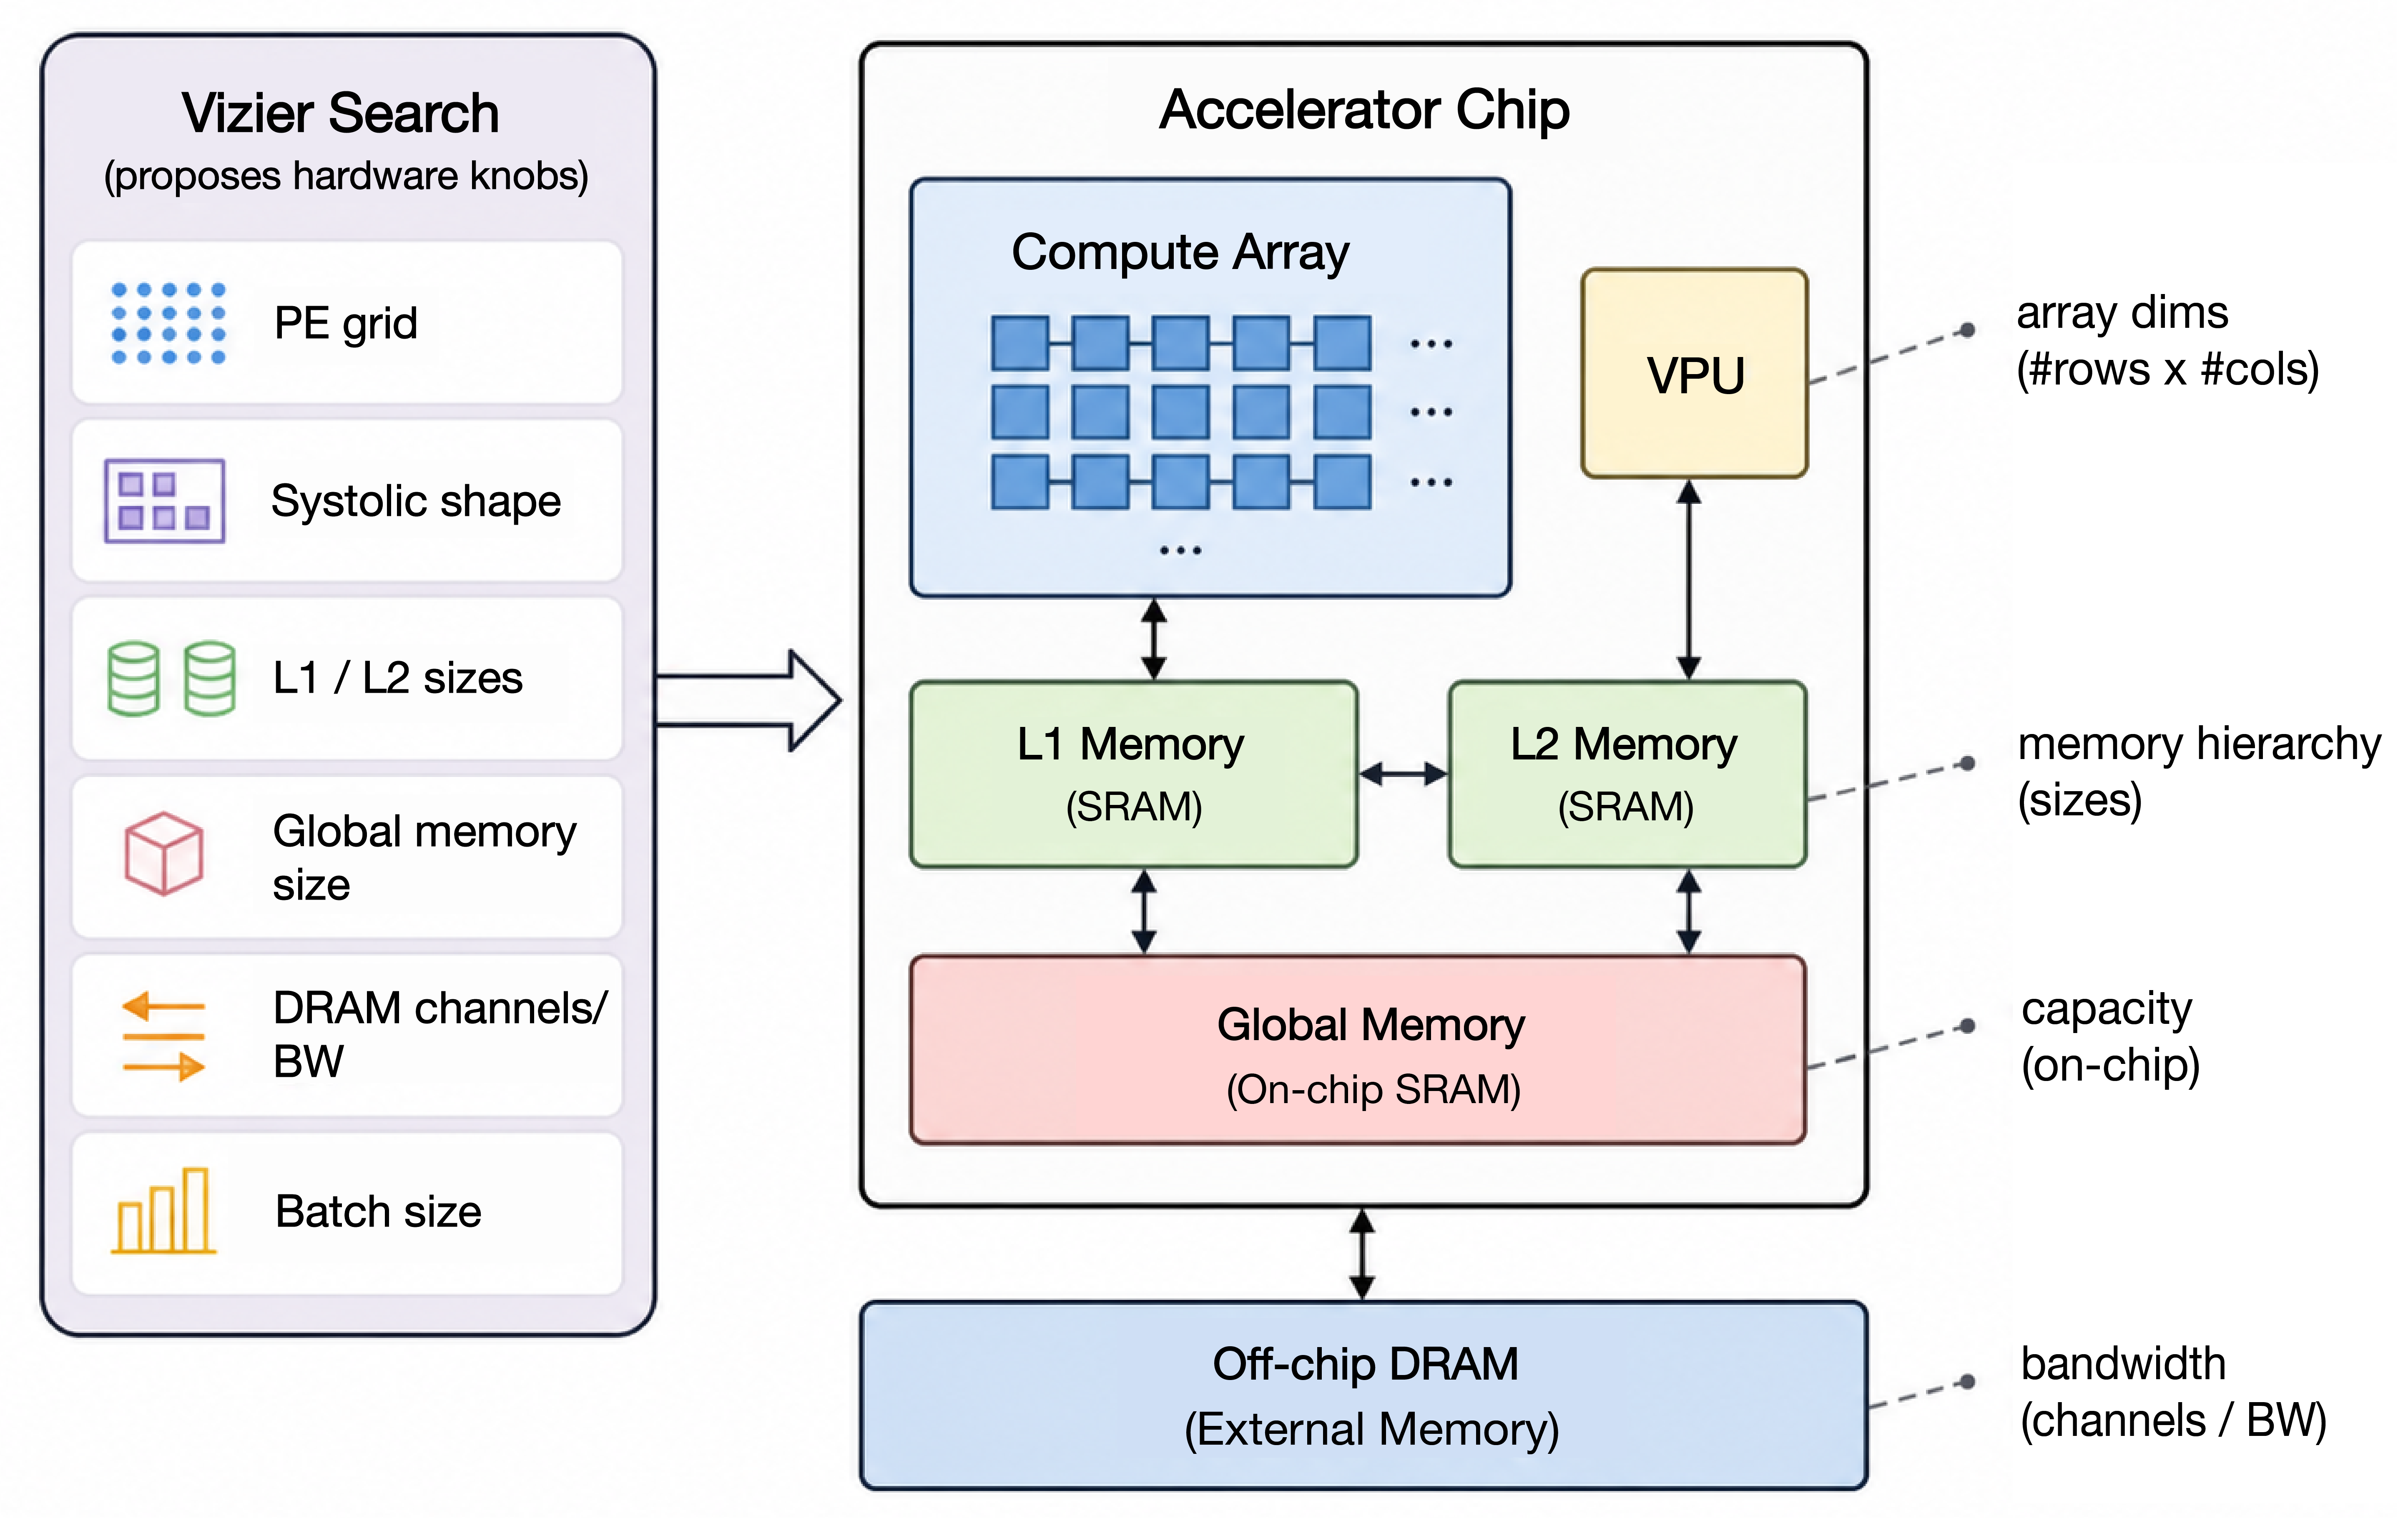
\includegraphics[width=0.7\linewidth]{figs/hardware_layout_v4.png}
%     \caption{The accelerator datapath configuration. Processing elements (PEs) are arranged in a grid connected by a mesh network. Each PE contains a systolic array for matrix operations, a vector processing unit (VPU) for non-MAC operations, and private or shared L1/L2 memory. A Global Memory serves as the on-chip scratchpad shared across all PEs.}
%     \label{fig:pipeline}
% \end{figure}
% \label{app:vizier}
% \begin{table}[h]
% \centering
% \caption{Vizier search parameter groups and ranges: initial small search vs.\ expanded V1-wide search.}
% \label{tab:vizier_search_space}
% \resizebox{\textwidth}{!}{%
% \begin{tabular}{llll}
% \toprule
% \textbf{Group} & \textbf{Parameter} & \textbf{Small (initial)} & \textbf{LLM-V1-wide} \\
% \midrule
% \multirow{16}{*}{\textbf{A — Hardware datapath (16 params)}}
%  & \texttt{PEs\_x\_dim}                & pow2 in $\mathbf{4 \ldots 32}$                          & pow2 in $\mathbf{1 \ldots 256}$                        \\
%  & \texttt{PEs\_y\_dim}                & pow2 in $\mathbf{4 \ldots 32}$                          & pow2 in $\mathbf{1 \ldots 256}$                        \\
%  & \texttt{Systolic\_array\_x}         & pow2 in $\mathbf{4 \ldots 32}$                          & pow2 in $\mathbf{4 \ldots 128}$                        \\
%  & \texttt{Systolic\_array\_y}         & pow2 in $\mathbf{4 \ldots 32}$                          & pow2 in $\mathbf{4 \ldots 128}$                        \\
%  & \texttt{Vector\_unit\_multiplier}   & pow2 $1 \ldots 16$                                      & pow2 $1 \ldots 16$                                     \\
%  & \texttt{L1\_buffer\_config}         & \{Private, Shared\}                                     & \{Private, Shared\}                                    \\
%  & \texttt{L1\_input\_buffer\_size}    & pow2 $\mathbf{1\,\text{KB} \ldots 4\,\text{MB}}$        & pow2 $\mathbf{1\,\text{KB} \ldots 1\,\text{MB}}$       \\
%  & \texttt{L1\_weight\_buffer\_size}   & pow2 $\mathbf{1\,\text{KB} \ldots 4\,\text{MB}}$        & pow2 $\mathbf{1\,\text{KB} \ldots 1\,\text{MB}}$       \\
%  & \texttt{L1\_output\_buffer\_size}   & pow2 $\mathbf{1\,\text{KB} \ldots 4\,\text{MB}}$        & pow2 $\mathbf{1\,\text{KB} \ldots 1\,\text{MB}}$       \\
%  & \texttt{L2\_buffer\_config}         & \{Disabled, Private, Shared\}                           & \{Disabled, Private, Shared\}                          \\
%  & \texttt{L2\_input\_buffer\_mult.}   & pow2 $1 \ldots 128$                                     & pow2 $1 \ldots 128$                                    \\
%  & \texttt{L2\_weight\_buffer\_mult.}  & pow2 $1 \ldots 128$                                     & pow2 $1 \ldots 128$                                    \\
%  & \texttt{L2\_output\_buffer\_mult.}  & pow2 $1 \ldots 128$                                     & pow2 $1 \ldots 128$                                    \\
%  & \texttt{L3\_global\_buffer} (CGM)   & $\{0\} \cup$ pow2 $\mathbf{1 \ldots 64\,\text{MB}}$     & $\{0\} \cup$ pow2 $\mathbf{1 \ldots 256\,\text{MB}}$   \\
%  & \texttt{GDDR6\_channels}            & pow2 $\mathbf{1 \ldots 16}$ ($\to$ 64–1024 GB/s)        & pow2 $\mathbf{1 \ldots 32}$ ($\to$ 64–2048 GB/s)       \\
%  & \texttt{Native\_batch\_size}        & pow2 $\mathbf{1 \ldots 1024}$                           & pow2 $\mathbf{1 \ldots 256}$                           \\
% \midrule
% \multirow{3}{*}{\textbf{B — Compiler passes (3 params)}}
%  & \texttt{two\_pass\_softmax}         & \{disabled, enabled\}                                   & \{disabled, enabled\}                                  \\
%  & \texttt{tensor\_padding}            & \{disabled, enabled\}                                   & \{disabled, enabled\}                                  \\
%  & \texttt{datatype}                   & \{bfloat16, int8\}                                      & \{bfloat16, int8\}                                     \\
% \midrule
% \multirow{2}{*}{\textbf{C — V0 rematerialisation (2 params)}}
%  & \texttt{remat\_enabled}             & \{disabled, enabled\}                                   & \{disabled, enabled\}                                  \\
%  & \texttt{remat\_cost\_scale}         & \{0.1, 0.25, 0.5, 1.0, 2.0, 4.0\}                      & \{0.1, 0.25, 0.5, 1.0, 2.0, 4.0\}                     \\
% \midrule
% \multirow{4}{*}{\textbf{D — V1 joint-tiling (4 params)}}
%  & \texttt{pareto\_config\_count\_C}   & \{10, 50, 100, 250, 500, 1000\}                         & \{10, 50, 100, 250, 500, 1000\}                        \\
%  & \texttt{loop\_ordering\_strategy}   & \{weight\_stationary, output\_stationary, both\}        & \{weight\_stationary, output\_stationary, both\}       \\
%  & \texttt{pareto\_pruning\_strategy}  & \{tmax\_workingset, tmax\_tmin, tmin\_workingset\}      & \{tmax\_workingset, tmax\_tmin, tmin\_workingset\}     \\
%  & \texttt{tile\_workingset\_modeling} & \{fixed, config\_dep\}                                  & \{fixed, config\_dep\}                                 \\
% \midrule
% \multirow{4}{*}{\textbf{Post-Vizier gates (filter, not search)}}
%  & \texttt{MIN\_TOTAL\_MACS}           & \multicolumn{2}{l}{$32{,}768$ ($4{\times}4{\times}4{\times}4{=}256$ lower physical, 32K gate)} \\
%  & \texttt{MAX\_TOTAL\_MACS} cap       & none — implicit $\leq 32{\times}32{\times}32{\times}32 \approx 1\,\text{M}$ & $1{,}048{,}576$ explicit cap \\
%  & Implied total\_MACs reach           & ${\approx}\,256 \ldots 1\,\text{M}$                     & $256 \ldots 1{,}048{,}576$ (post-cap)                  \\
%  & Implied DRAM BW reach               & $64 \ldots 1{,}024$ GB/s                                & $64 \ldots 2{,}048$ GB/s                               \\
% \bottomrule
% \end{tabular}%
% }
% \end{table}


\subsection{Why We Are Confident in the Software Side}
\label{app:sw_confidence}

The software claim is that the schedule the program commits to is the schedule
that runs, and that its optimality is bounded rather than asserted. Five
independent checks support it, ordered from strongest to weakest.

\paragraph{The committed schedule executes byte-exactly in RTL.}
The full DeepSeek-V3 schedule is compiled into a $1{,}383$-instruction event tape
and executed on a cycle-accurate SystemVerilog engine under Verilator
(\cref{sec:rtl_validation}). The run completes with \textbf{zero} capacity
violations; the RTL peak on-chip occupancy equals the analytical prediction
\emph{exactly} at $7{,}602{,}176$~bytes; and the total cycle count lands within
$+0.000001\%$ of the rounded LP objective. This is the strongest form of the
claim available without silicon: the plan is not merely feasible on paper, it is
executable byte-for-byte on hardware that enforces the capacity constraint at
every step.

\paragraph{The checker is live, not vacuous.}
A validation suite is only meaningful if it can fail. We therefore replay a
deliberately over-committed tape, and the capacity checker flags exactly one
violation. A test that never fails proves nothing; this one fails when it should.

\paragraph{Optimality is bounded, not claimed.}
Every reported design is a certified achievable point, and we also solve the
relaxation to obtain a bound no design in the model can beat. The pair brackets
the unknown optimum (\cref{sec:certified_gap}), and the bracket tightens to
${\sim}13.5\%$ in the high-batch regime. Where the bracket is wide we say so
rather than reporting the achievable alone.

\paragraph{Rounding is feasibility-preserving and independently validated.}
Relaxed selectors are rounded by enumeration over the physically integral
choices, and no pin that would violate a constraint is ever committed. Each
rounded design is re-solved and checked against the constraint set independently
of the solver that produced it, with residuals at the $10^{-13}$ level. We never
report a relaxed objective as an achievable result.

\paragraph{One search setting produces every number.}
All serving results come from a single documented search configuration
(\cref{app:coeff_provenance}), including the baselines, so no comparison mixes a
finely searched design against a coarsely searched baseline. Cross-table
consistency is verified at the shared operating point.

\paragraph{What this does not establish.}
RTL cycle counts are not used as an absolute oracle: the analytical per-layer
cache floors are conservative by $192\times$ to $2475\times$, so RTL evidence is
scoped to schedule realizability, memory legality, and utilization
\emph{mechanisms}. We make no claim that the simulated datapath is a
performance-optimal implementation.

\subsection{Why We Are Confident in the Hardware Side}
\label{app:hw_confidence}

The hardware claim is narrower and we state it precisely: the cost model that
costs silicon is faithful enough that a design certified against it would be
buildable. Design-space-exploration frameworks are conventionally validated
three ways, against measured taped-out chips, against post-synthesis extraction,
and against other frameworks~\citep{mei2021zigzag}. We have all three.

\paragraph{Against post-synthesis extraction: the area coefficient and its
functional form.}
We implement the scored datapath as synthesizable RTL and push it through
OpenROAD to placement at the ASAP7 $7$~nm predictive PDK
(\cref{sec:asap7}). Extracted cell area fits
$A = 82.08\,\mathrm{MACs} - 206.5\ \mu\mathrm{m}^2$ with $R^2 = 0.999999$, and
area per MAC varies by only $0.46\%$ across a $16\times$ range in MAC count. The
second number matters more than the first: the program assumes area is
\emph{linear with a size-independent slope}, and that is exactly what a placed
datapath exhibits. The coefficient we use is bracketed from below by extracted
cell area and from above by our own conservative floorplan.

\paragraph{Against shipped silicon: the energy coefficient.}
Our compute-energy coefficient corresponds to $0.40$~pJ per INT8 operation. Whole
chip figures for shipped accelerators are $0.35$ (H100), $0.64$ (A100) and
$1.27$~pJ/op (TPU-v4i), and an array-only coefficient must sit at or just below
whole-chip values. It does. We additionally measured the precision-energy ratio
directly rather than assuming it, and the measurement corrected our analytic
estimate in both directions (\cref{sec:energy_coeff}).

\paragraph{Against other frameworks: the mapping data.}
Every per-tile latency and byte count entering the program is measured Timeloop
Pareto data, not an analytic surrogate.

\paragraph{Manufacturability is enforced, not audited.}
The six pre-RTL gates are rows of the program rather than post-hoc screens, so a
gate can only ever be reported as satisfied. Every design in this paper passes
all six.

\paragraph{What this does not establish.}
We have not taped out, and we do not run clock-tree synthesis or routing, so we
make no claim about achievable clock frequency in silicon. Absolute power from
our own flow remains an upper bound rather than a prediction: an ungated tile
driven by uncorrelated data on a predictive PDK reports roughly three times our
coefficient, and we therefore anchor the coefficient to measured silicon rather
than to our own synthesis. The gating measurement in particular is not yet
trustworthy and no clock-gating decision is scored in the program as a result.
